\documentclass[12pt,a4paper]{article} 
\usepackage[T1]{fontenc}
\usepackage[francais]{babel}
\usepackage[latin1]{inputenc}
\usepackage{amsmath}
\usepackage{amssymb} %pour des symboles mathematique
\usepackage{graphicx} 
\usepackage{epstopdf} %pour utiliser les .eps
\usepackage{url}
\usepackage{fancyhdr}
\usepackage{fullpage}
\usepackage{array}
\usepackage[table]{xcolor} %pour les couleurs
\usepackage{multicol}
\usepackage[babel=true]{csquotes} %pour les citations
\usepackage{hyperref}
\usepackage{float} 
\usepackage{adjustbox} %pour resizer les tableaux

%%%% pour l'insertion de code %%%%%
\usepackage{listings}
\usepackage{color}

\definecolor{dkgreen}{rgb}{0,0.6,0}
\definecolor{gray}{rgb}{0,0,0}
\definecolor{mauve}{rgb}{0,0,0}

\lstset{emph={%  
    float, %
    },emphstyle={\color{gray}\bfseries}%
}%

\lstset{frame=tb,
  language=Matlab,
  aboveskip=3mm,
  belowskip=3mm,
  showstringspaces=false,
  columns=flexible,
  basicstyle={\small\ttfamily},
  numbers=none,
  numberstyle=\tiny\color{gray},
  keywordstyle=\color{black},
  commentstyle=\color{dkgreen},
  stringstyle=\color{black},
  identifierstyle=\color{mauve},
  breaklines=true,
  breakatwhitespace=true
  tabsize=3
}

%%%%%%%%%%%%%%%%%%%%%%

%\pagestyle{myheadings}
%\markright{Tableau blanc interactif}

\title{\LARGE \textbf{Project - The Game Cube\textregistered}\\
	\bigskip
	\bigskip
	\large Technologies for human-computer interactions}
\author{Aina Rasolonjatovo Alain Nary Andriambelo \\ Samuel Constantino}
\date{Spring 2014}

\parindent=0cm
\parskip=6pt

\begin{document}
	\maketitle

%%%%%%%%%%%%%%%%%%%%%%%

\section{Introduction}

The goal of this project is to build a game exploring original human-machine interactions. For that, we used a galvanic skin response (GSR) sensor as the main mean of interaction and the \texttt{Blender} 3d software to create the game. In our project, we use the GSR data - which measures skin conductance - as an indicator for stress and arousal. The goal of the game is for the player to manage her stress level and relax. 

\section{Project}

\subsection{Sensor data}

We started from the premise that the GSR sensor could be used as an indicator of excitement. Psychological arousal is linked with nervous activity that changes skin conductance. However, data from the GSR sensor isn't necessarily stable and skin conductance is subject to sudden changes (spikes) that doesn't reflect a general state of being.

In our game, we used a statistical analysis technique called \textbf{moving average} to smooth out the data. The advantage of the moving average is that it reduces the impact of spikes but still preserves long-term tendencies, similarly to a low-pass filter. This technique is usually used in finance and economy to represent trends over time, which is what we want with real-time acquisition of data. More precisely, we use a weighted moving average (WMA) which gives more importance to the oldest data and prevent influence from sudden spikes. It has the following formula : 

\begin{equation}
\text{WMA} = \frac{n * p_n + (n - 1) * p_{n-1} + ... + 1 * p_{1}}{n + (n-1) + ... + 1}
\end{equation}

Where $n$ is the number of data in a queue, $p_x$ is some GSR value at point $x$ in the queue and $p_n$ is the oldest data in the queue. Our moving average is calculated for each new received data by adding it to a queue of size $n=20$.

Here is an illustration of the smoothing done by moving average\footnote{Image taken from : \\ \hyperref[]{http://support2.dundas.com/OnlineDocumentation/WinChart2003/WeightedMovingAverage.html}} :

\begin{figure}[H] 
\centering
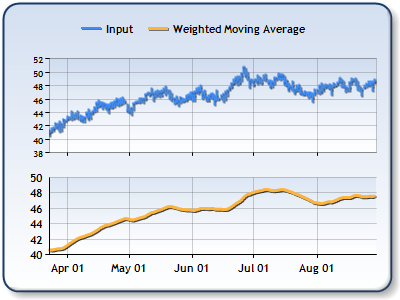
\includegraphics{WeightedMovingAverage.png}
\caption{Exemple of smoothing with weighted moving average.}
\end{figure}

The disadvantage of this technique is that there is a slight delay when trends shift, because the first few points do not have enough weight to influence the average yet.

\subsection{Game design}

The game consists of a cube rotating in the middle of the screen. The cube rotates according to the player's state. Getting excited results in a fast acceleration while being calm makes the cube slow down. By controlling her ``emotions'' (or at least her excitation), the player can then control the speed of the rotation.

%2 modes
The game has two modes of play, Relaxation mode and Challenge mode. 

The Relaxation mode consist only of a rotating cube inside an environment without time limit. There is no objective in this mode. It can be used as a introduction to the game, for familiarization.

%Challenge mode : introduction
The Challenge mode is about winning as much point as possible by controlling the cube rotation during missions during a time limit. Since the game is about controlling the stress of a player, two elements are used during the game : Mission where the player have to change his stress to have benefices and Event that disrupt the player.

%Challenge mode : Mission
In the Challenge mode, the missions are based on controlling the speed of the cube, such as not exceed a given speed value. Completing a mission grants the player points for her score, and extends the time before the game is over. Failing a mission won't have any effect, beside the time lost during the mission. Up to two missions can appears at the same time. After the time limit is elapsed, the game is over. The mission are randomized  to prevent prediction.

%Challenge mode : Event
While playing the Challenge mode some events occur. The interface or the cube's environment are modified in order to destabilize the player, which can make some missions harder. For example the cube can suddenly stop moving, although that the stress of the player still affects the results of the missions. The events occur randomly and may not happen at all during a game.

%way to understand how game works
%how rythme works
%relax and sooth 
%
%challenge mode,
%time limit, playing as long as possible
%win more time by completing missions
%once finished, score (calculated according to missions)
%mission types - 
%slow down, not variate, etc
%randomized mission in a shuffled list (to prevent many repetitions)
%special events to distract player - jump scare 


\subsection{Blender}

%send data over socket
At the start of the game Sockets are used between blender and the GSR device to establish a connection. We use the UDP protocol since the data from the GSR to the game is numerous. Unlike the TCP/IP protocol there is no problem if some data is lost and no synchronizations are required. The only data sent by the game to blender is a starting and stopping order to receive data.

%movement camera, 

%cube
The cube is a mesh cube that has a modifier applied to it. It consists of a sphere "expended" to the border of the cube, to every direction so that the corner and the edges are smoother.

HUD position

style

%%%%%%%%%%%%%%%%%%%%%%%%%%%%%%%%%%%%%%%%%%%%%%%%%%%%%%%%%%%%%%

\section{Evaluation}

image jeu 

objective : control emotions linked to stress

contrôle du jeu - player input
se calmer - peu être facile... ou pas
s'exciter en parlant
- difficulté jeu sans direct input

game plays better without player
because point of game is to be stable
(human hard to stay stable)
(because excitement; because sensor - transpiration?)

with experience, understand how can manipulate arousal
talking
closing eyes
focus on cube - can reduce - calm

\section{Conclusion}



\end{document}